\documentclass[handout]{beamer}
\usepackage{amsmath,amssymb,amsthm}
\usepackage[utf8]{inputenc}
\usepackage[russian]{babel}
\usepackage{alltt}
\usepackage{xcolor}
\usepackage{hyperref}
\usepackage{adjustbox}
\usepackage{minted}
\usepackage{graphicx}
\graphicspath{{pictures/}}
\usepackage{ragged2e}
\usepackage{minted}
\usepackage{caption}
\usepackage{xmpmulti}
\usepackage{tcolorbox}

\usepackage[most]{tcolorbox}

\newtcolorbox[auto counter]{pabox}[1]{%
    colback=white,
    colframe=structure.fg,
    colbacktitle=white!90!structure.fg,
    coltitle=black,
    fonttitle=\bfseries, 
    title=Важное,
    enhanced,
    attach boxed title to top left={yshift=0mm, xshift=0cm}
}

\newlength\someheight
\setlength\someheight{3cm}

\definecolor{urlcolor}{HTML}{3205FF}

\usetheme{Montpellier}
\usecolortheme{seahorse}
\logo{
\includegraphics[width=0.2\textwidth]{img/logo.png}}

\title{Мастер-класс}
\subtitle{Реализация простого аналога Minecraft\\на Python помощью движка Ursina}
\author{Попов Никита \\ \href{mailto:me@l4zzur.ru}{me@l4zzur.ru}}
\institute{Международная школа программирования и математики Алгоритмика}
\date{19 августа 2023 года}

\begin{document}

    \section{Титульный лист}
    \begin{frame}
        \titlepage
    \end{frame}

    \section{Знакомство}
    \begin{frame}{Спикер - Никита}
        \begin{columns}
            \begin{column}{0.4\textwidth}
                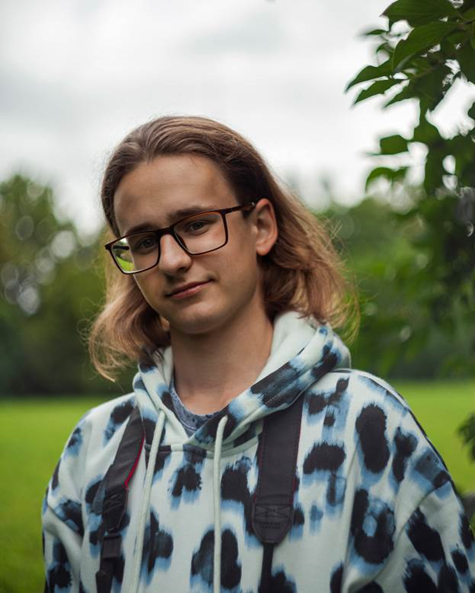
\includegraphics[width=\textwidth]{img/me.png}
            \end{column}
            \begin{column}{0.6\textwidth}
                \begin{itemize}
                    \item Образование – специалист по компьютерной безопасности;
                    \item Начал с создания ботов для Telegram и использования разнообразных библиотек для Python;
                    \item Преподаватель Python в Алгоритмике;
                    \item В свободное время занимаюсь изучением PyQt, написанием обертки Monstercat API.
                \end{itemize}
            \end{column}
        \end{columns}
    \end{frame}

    \begin{frame}{Почему именно Python?}
        \begin{tcolorbox}[colback=blue!5,colframe=blue!75!black]
           Python - это язык программирования близкий к естественному человеческому языку и легко читаемый. Python позволяет решать разнообразные задачи.
        \end{tcolorbox}
        \begin{columns}
            \begin{column}{0.37\textwidth}
                Множество обучающего материала и большое сообщество
                \newline \newline
                Легкость и понятность кода
            \end{column}
            \begin{column}{0.25\textwidth}
                \begin{center}
                    
\includegraphics[width=\textwidth]{img/Python_logo_icon.png}
                \end{center}
            \end{column}
            \begin{column}{0.37\textwidth}
                Большое количество библиотек для разных задач
                \newline \newline
                Кроссплатформенность
            \end{column}
        \end{columns}
    \end{frame}

    \begin{frame}[fragile]
        \frametitle{Пример кода}
        \scriptsize
        \rule{\textwidth}{1pt}
        \begin{minted}[autogobble]{python}
            # Импортируем модуль random, который позволяет генерировать случайные числа
            import random
            # Создаем переменную number и присваиваем ей случайное число от 1 до 10
            number = random.randint(1, 10)
            # Выводим сообщение на экран
            print("Я загадал число от 1 до 10. Попробуй угадать!")
            while True: # Создаем бесконечный цикл
                # Запрашиваем у пользователя ввод числа
                guess = input("Введи свой вариант: ") 
                guess = int(guess) # Преобразуем введенное значение в целое число
                if guess == number: # Сравниваем введенное число с загаданным
                    # Если числа равны, то выводим сообщение об успехе и выходим из цикла
                    print("Ура, ты угадал!")
                    break
                # Иначе, если введенное число меньше загаданного, то выводим подсказку
                elif guess < number:
                    print("Нет, мое число больше.")
                # Иначе, если введенное число больше загаданного, то выводим подсказку
                else:
                    print("Нет, мое число меньше.")
        \end{minted}
        \rule{\textwidth}{1pt}
    \end{frame}

    \section{Minecraft}
    \begin{frame}{Почему именно Minecraft?}
        \begin{columns}
            \begin{column}{0.5\textwidth}
                Minecraft - это компьютерная игра в жанре песочницы, созданная шведским программистом Маркусом Перссоном и выпущенная его студией Mojang. Игроки могут свободно строить и разрушать блоки, создавать различные предметы и взаимодействовать с другими игроками в многопользовательском режиме.
            \end{column}
            \begin{column}{0.5\textwidth}
                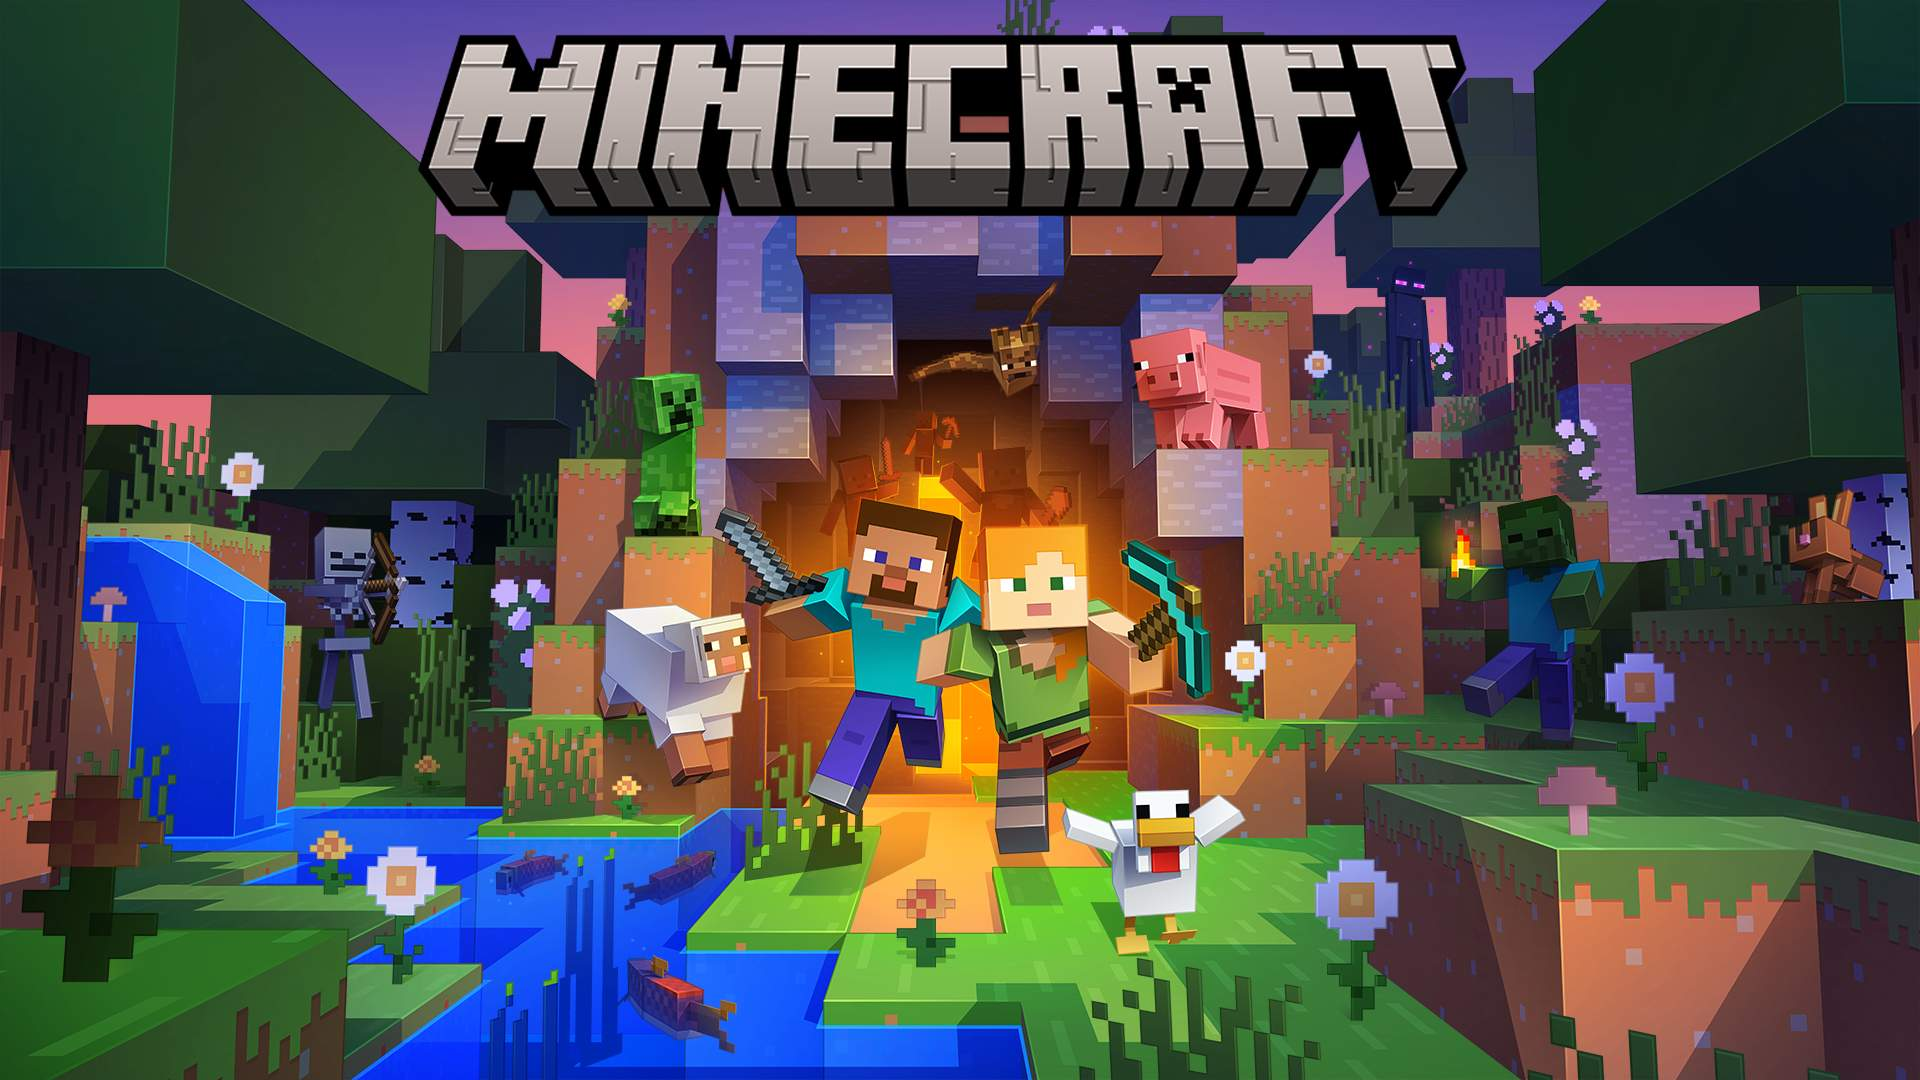
\includegraphics[width=\textwidth]{img/minecraft.jpg}
            \end{column}
        \end{columns}
    \end{frame}

    \begin{frame}{История создания}
        \begin{columns}
            \begin{column}{0.42\textwidth}
                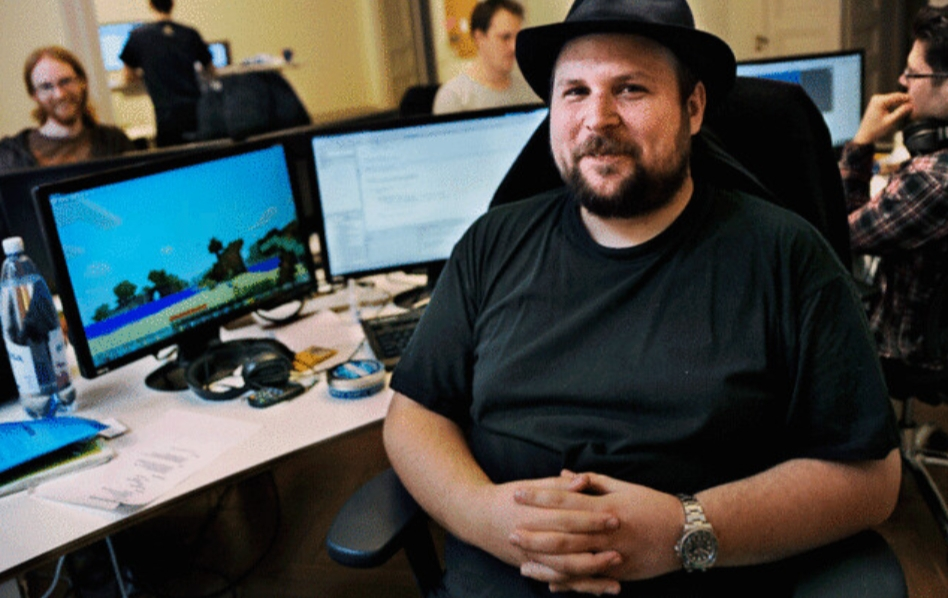
\includegraphics[width=\textwidth]{img/markus.jpg}
            \end{column}
            \begin{column}{0.7\textwidth}
                \begin{itemize}
                    \item Minecraft был создан шведским программистом Маркусом Перссоном, известным под псевдонимом Notch.
                    \item Перссон начал работу над игрой в мае 2009 года, вдохновившись такими играми, как Dwarf Fortress, Dungeon Keeper и Infiniminer.
                    \item Первая версия игры, называемая Classic, была опубликована на официальном сайте в июне 2009 года. Она была бесплатной и позволяла игрокам строить из разных блоков в режиме креатива.
                \end{itemize}
            \end{column}
        \end{columns}
    \end{frame}

    \begin{frame}{Cave Game}
        \begin{columns}
            \begin{column}{0.5\textwidth}
                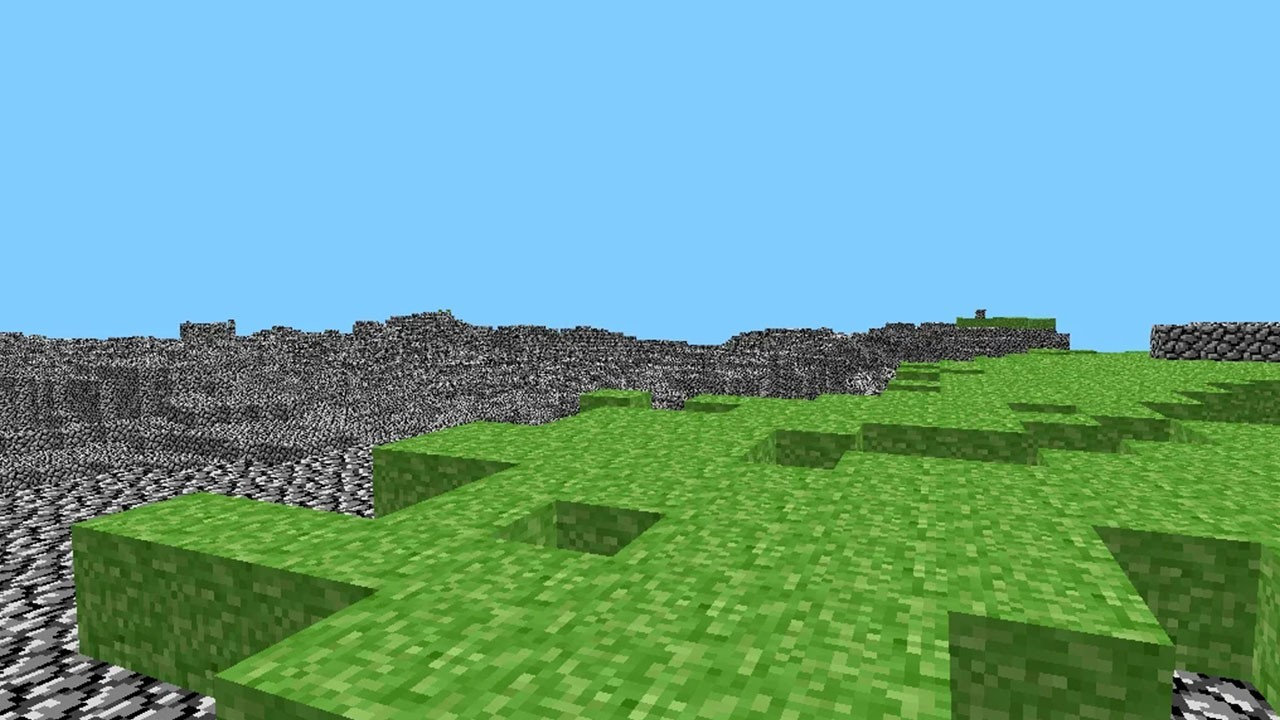
\includegraphics[width=\textwidth]{img/mine1.jpg}
            \end{column}
            \begin{column}{0.5\textwidth}
                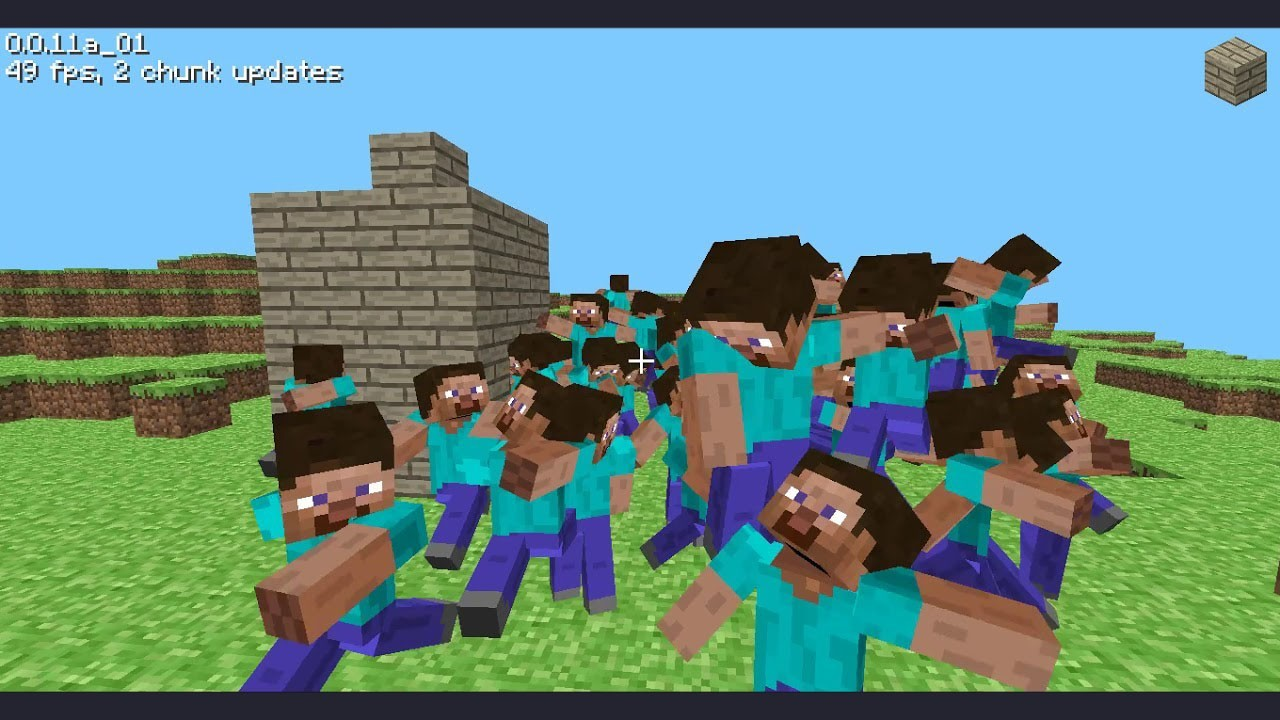
\includegraphics[width=\textwidth]{img/mine2.jpg}
            \end{column}
        \end{columns}
    \end{frame}

    \section{Игровые движки}
    \begin{frame}{Разнообразие движков}
        \begin{columns}
            \begin{column}{0.33\textwidth}
                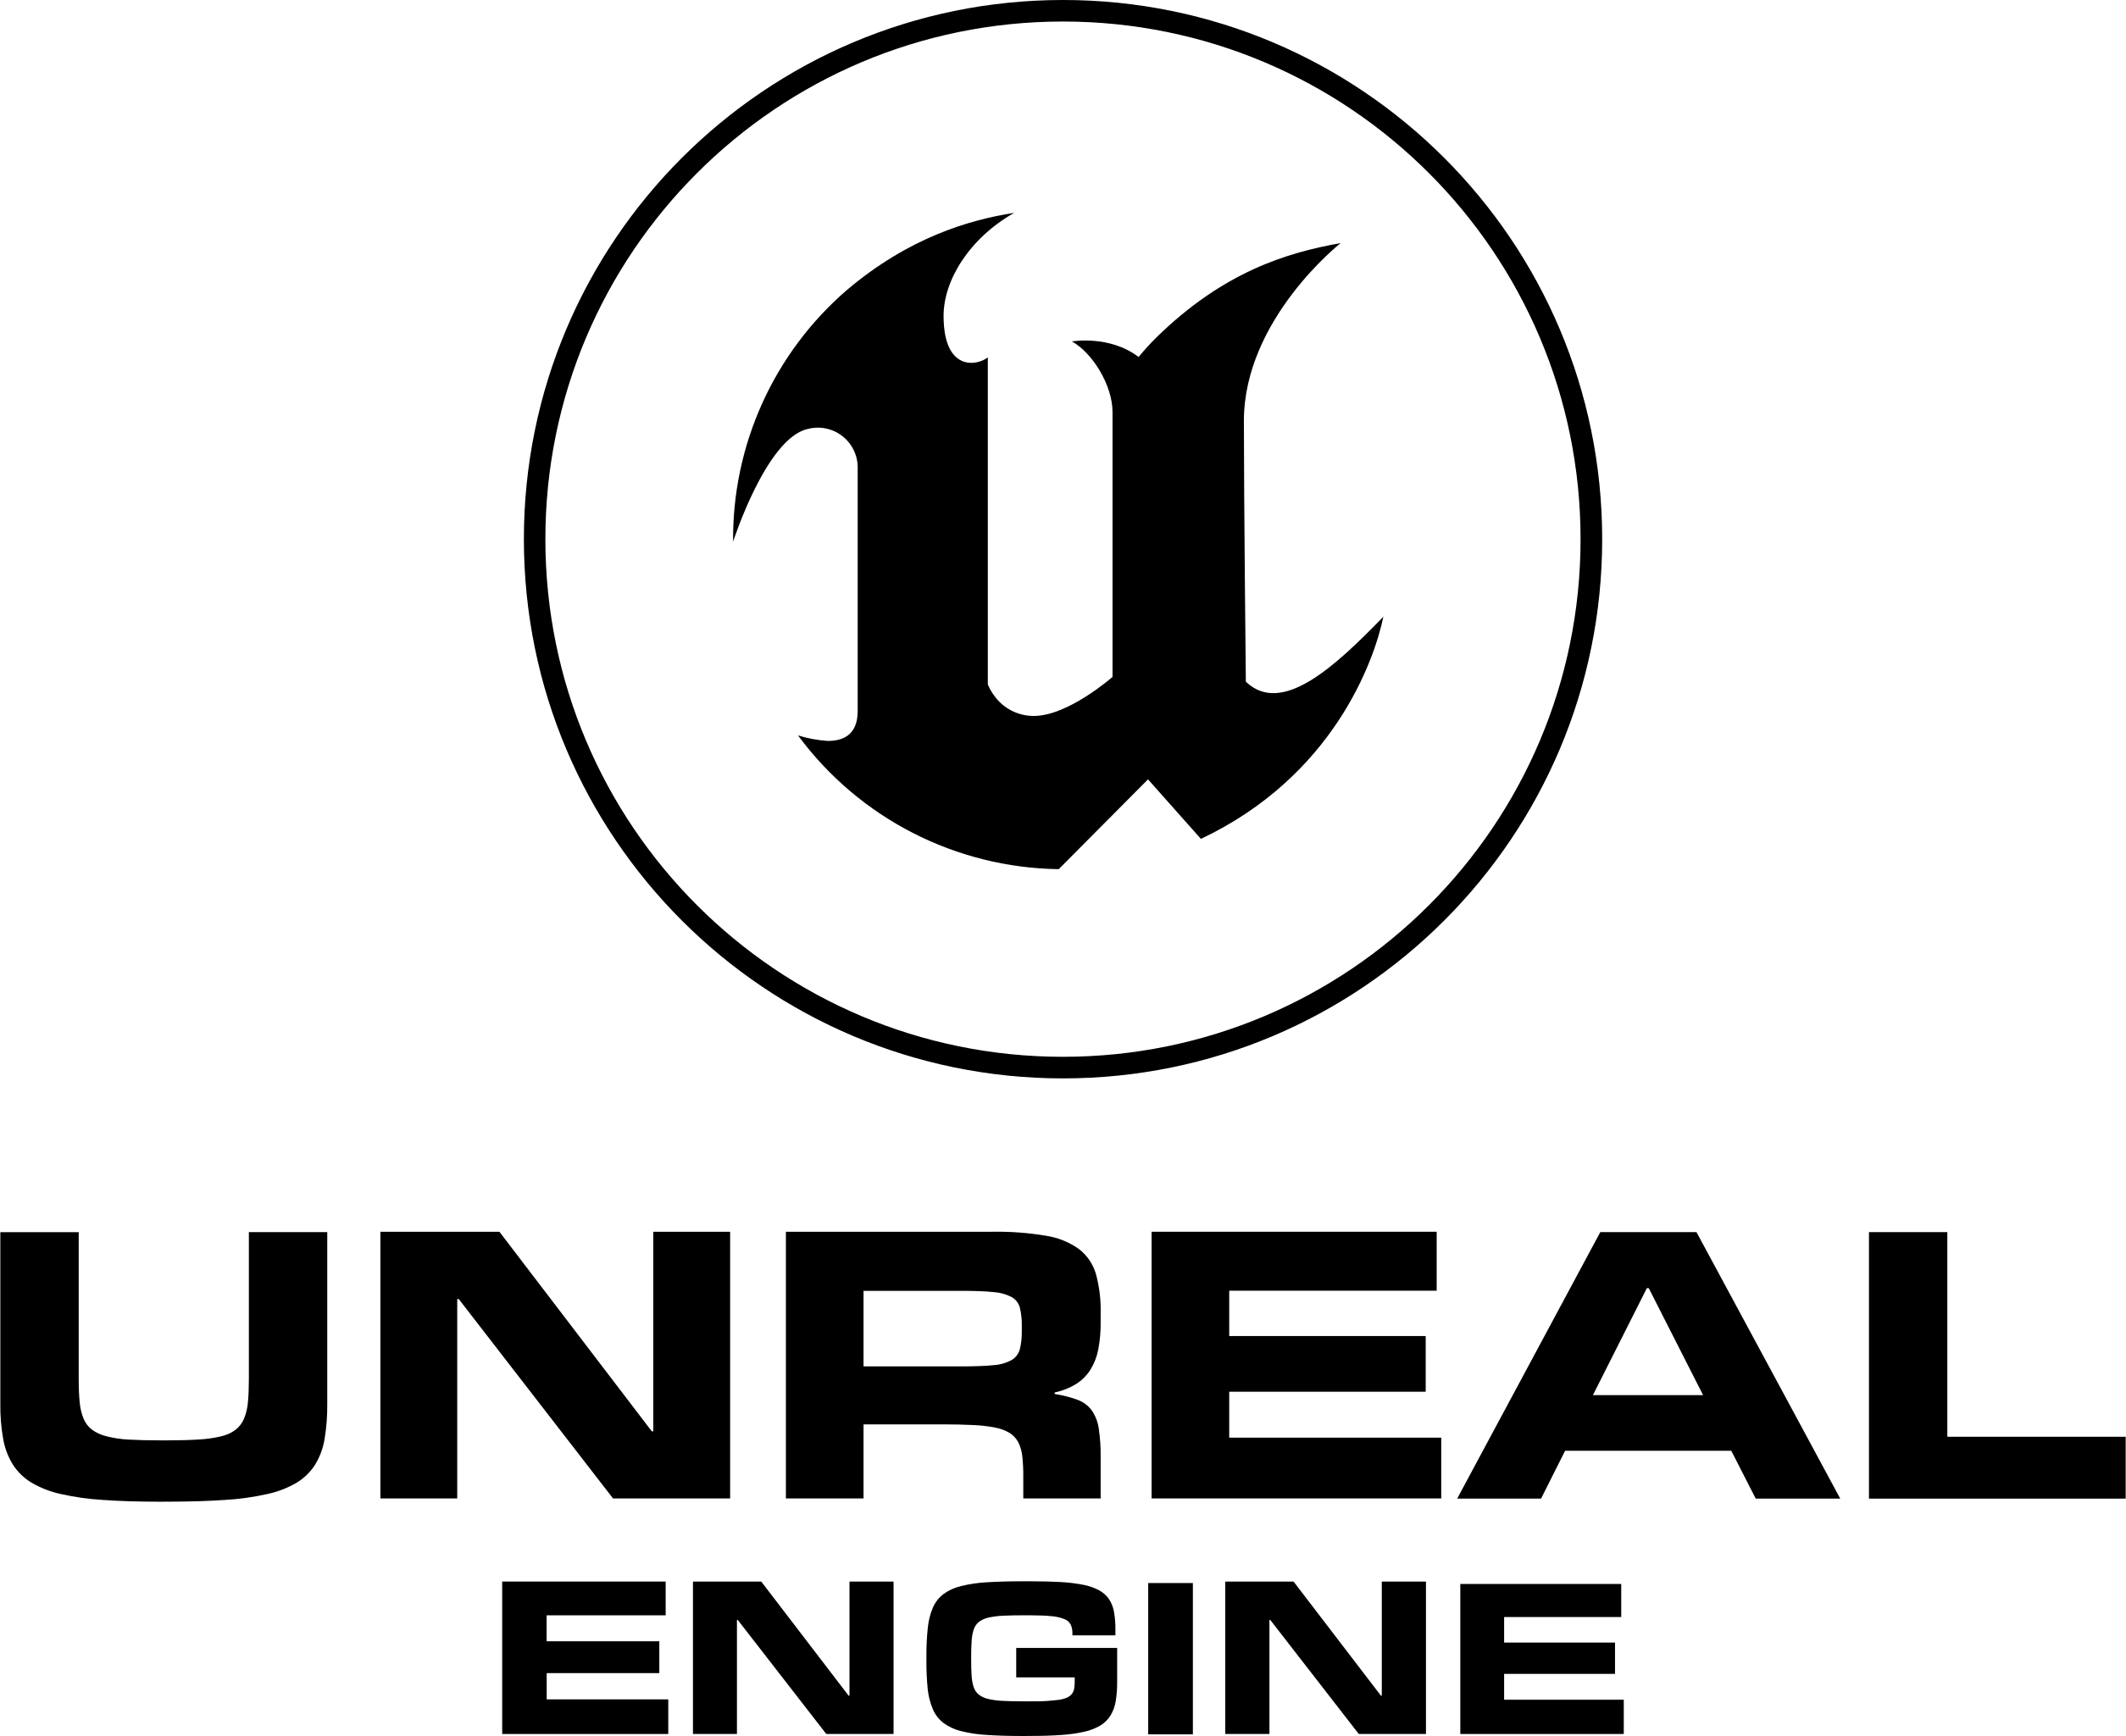
\includegraphics[width=\textwidth]{img/ue.png}
            \end{column}
            \begin{column}{0.33\textwidth}
                
\includegraphics[width=\textwidth]{img/unity.png}
            \end{column}
            \begin{column}{0.3\textwidth}
                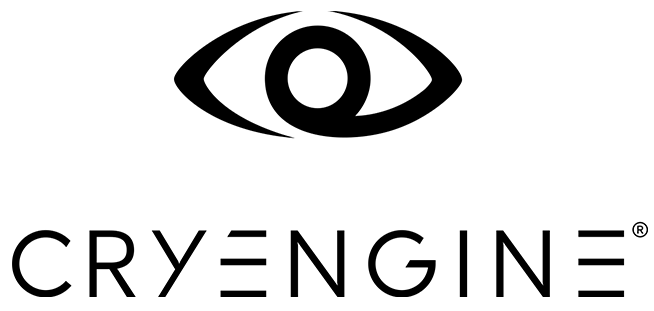
\includegraphics[width=\textwidth]{img/cryengine.png}
            \end{column}
        \end{columns}
    \end{frame}

    \begin{frame}{Движок Ursina}
        \begin{tcolorbox}[colback=blue!5,colframe=blue!75!black]
           Движок - это программа или набор программ, которые облегчают создание игр или других интерактивных приложений. 
        \end{tcolorbox}
        \begin{tcolorbox}[colback=blue!5,colframe=blue!75!black]
           Ursina - это движок для создания 2D, 3D-игр на Python. С его помощью мы сможем создать свой собственный мир Minecraft, добавлять объекты, текстуры, звуки, анимацию и логику игры.
        \end{tcolorbox}
    \end{frame}

    \begin{frame}{Примеры}
        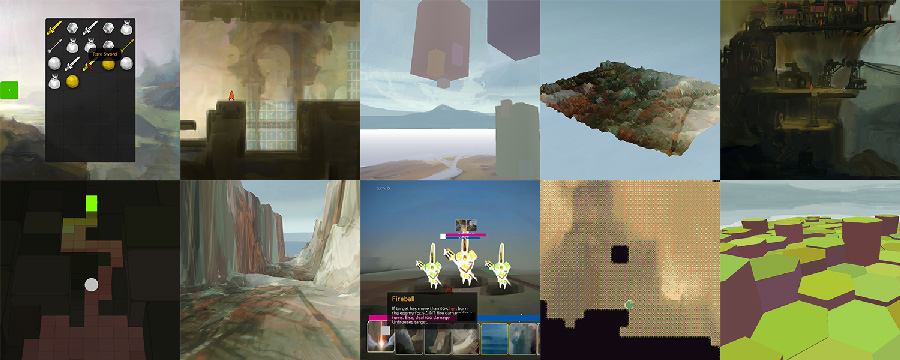
\includegraphics[width=\textwidth]{img/made_with_ursina.jpg}
        \begin{justify}
            2D-игры, 3D-игры, приложения, визуализации, вы можете сделать все, что захотите, с помощью Ursina.
        \end{justify}
    \end{frame}

    \begin{frame}{Современный интерфейс}
        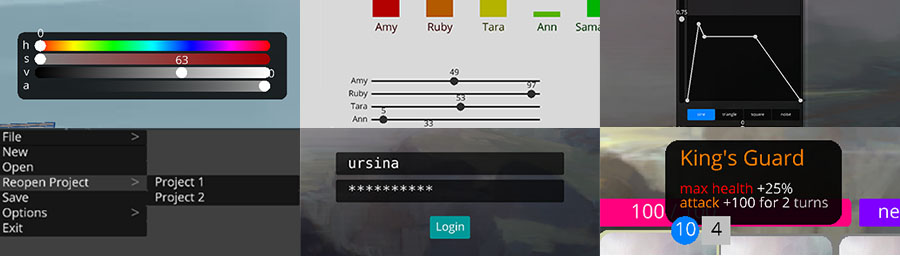
\includegraphics[width=\textwidth]{img/ursina_ui_banner.jpg}
    \end{frame}


    \begin{frame}{Преимущества Ursina}
        \begin{itemize}
            \item Ursina работает на Python.
            \item Ursina имеет современный дизайн и интерфейс. Ursina также имеет встроенные элементы управления для камеры, мыши и клавиатуры.
            \item Ursina бесплатен и открыт для изменений. Ursina распространяется под лицензией MIT, которая позволяет использовать Ursina для любых целей.
        \end{itemize}
    \end{frame}

    
    \begin{frame}{Тестовое приложение}
        \begin{justify}
            Попробуй запустить тестовый скрипт \texttt{sample.py}. \\ \textit{Чтобы управлять камерой зажми правую кнопку мыши и тяни мышь в разные стороны!}
        \end{justify}
        \begin{center}
            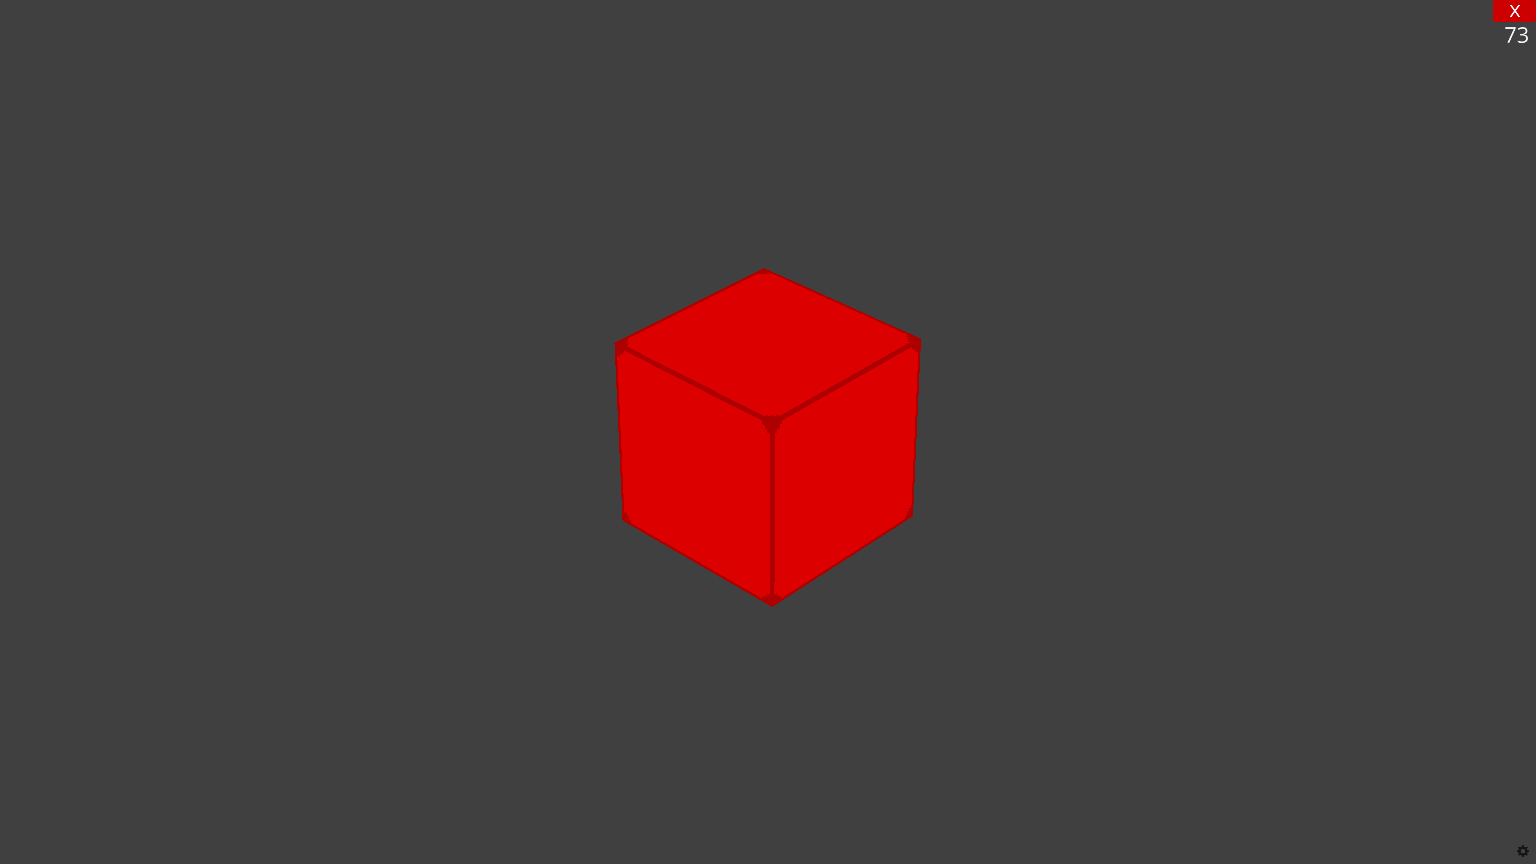
\includegraphics[width=0.7\textwidth]{img/0.png}
        \end{center}
    \end{frame}



    \section{Разработка клона Minecraft}
    \begin{frame}[fragile]{Шаблон проекта}
        \scriptsize
        \rule{\textwidth}{1pt}
        \begin{minted}[autogobble]{python}
            # Необходимые импорты
            from ursina import *
            
            # Инициализация окна игры
            app = Ursina() 
            
            # здесь будет описана игровая логика
            
            # Запускаем проект
            app.run()
        \end{minted}
        \rule{\textwidth}{1pt}
        \begin{center}
            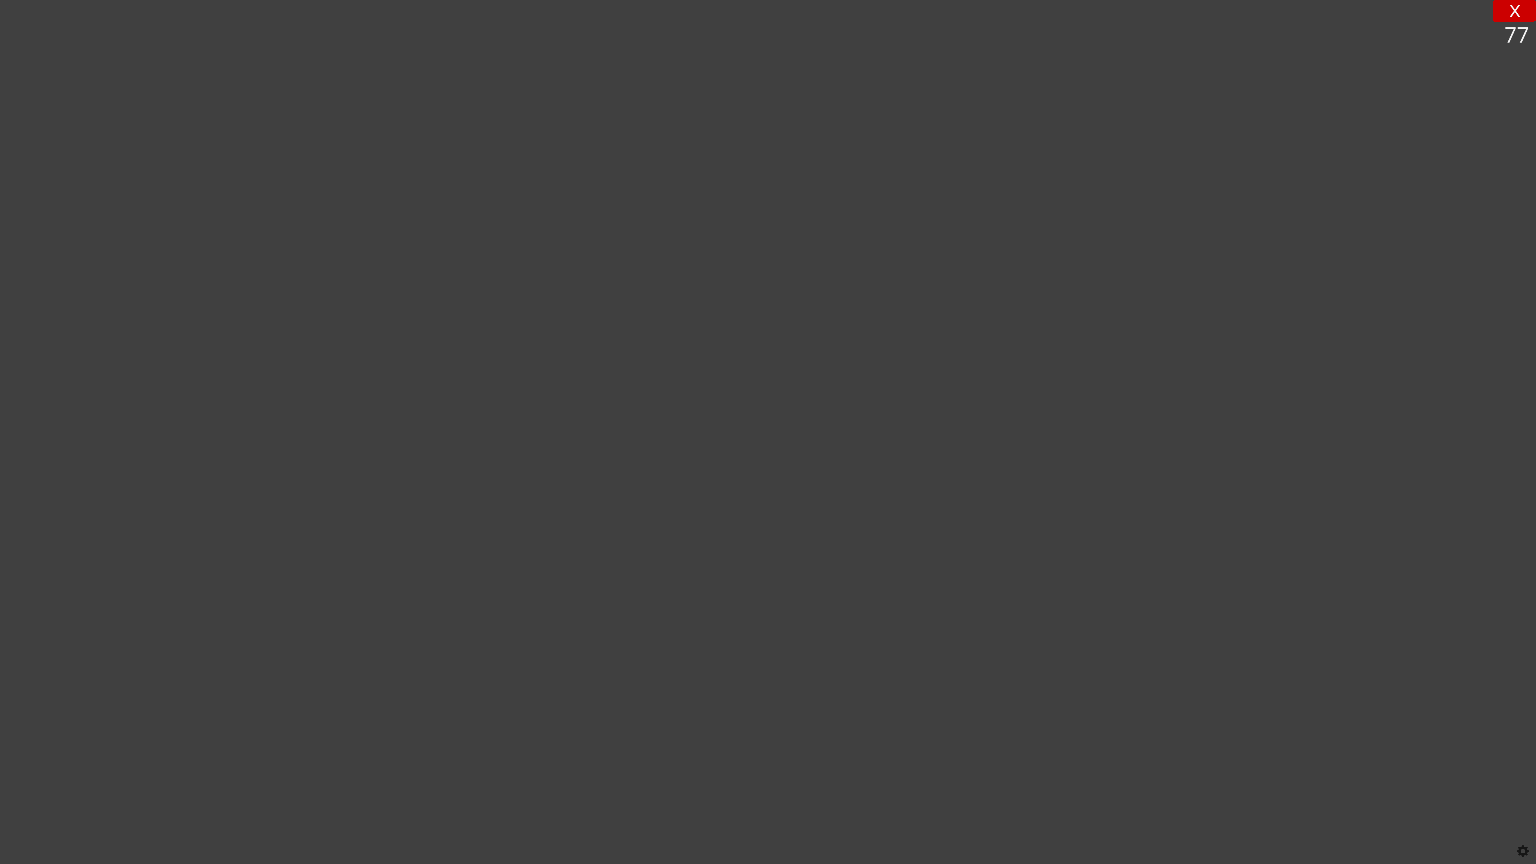
\includegraphics[width=0.4\textwidth]{img/1.png}
        \end{center}
    \end{frame}

    \begin{frame}[fragile]{Закрытие окна}
        \scriptsize
        \rule{\textwidth}{1pt}
        \begin{minted}[autogobble]{python}
            # Необходимые импорты
            from ursina import *
            
            # Инициализация окна игры
            app = Ursina()
            
            # Убираем кнопку закрытия окна
            window.exit_button.visible = False
            
            # Определяем функцию input с одним параметром key
            def input(key):
                # Проверяем, равна ли переменная key строке "q" или "escape"
                if key == "q" or key == "escape":
                    # Если да, то вызываем функцию quit, которая завершает работу приложения Ursina
                    quit()
            
            # Запускаем проект
            app.run()
        \end{minted}
        \rule{\textwidth}{1pt}
    \end{frame}


    \subsection{Entity}
    \begin{frame}{Определение}
        \begin{justify}
            Объект \textbf{Entity} - это основа для всех сущностей в игре. С его помощью можно создавать разные элементы игрового мира, например, фигуры (кубы, сферы, пирамиды и т.д.) или модели (персонажи, предметы и т.д.). Для наполнения карты воспользуемся им.
        \end{justify}
    \end{frame}

    \begin{frame}[fragile]{Код}
        \scriptsize
        \rule{\textwidth}{1pt}
        \begin{minted}[autogobble]{python}
            # Прошлый код
            ...
            
            # Создаем двойной цикл for, который повторяется 16 раз по переменным x и z
            for x in range(16): 
            	for z in range(16):
            	    # Создаем сущность в виде куба с белой текстурой и задаем ей 
                        # позицию в пространстве по координатам x, 0 и z
            	    Entity(model="cube", texture="white_cube", position=Vec3(x,0,z))
            
            # Запускаем проект
            app.run()
        \end{minted}
        \rule{\textwidth}{1pt}
    \end{frame}
    
    \begin{frame}{Результат}
        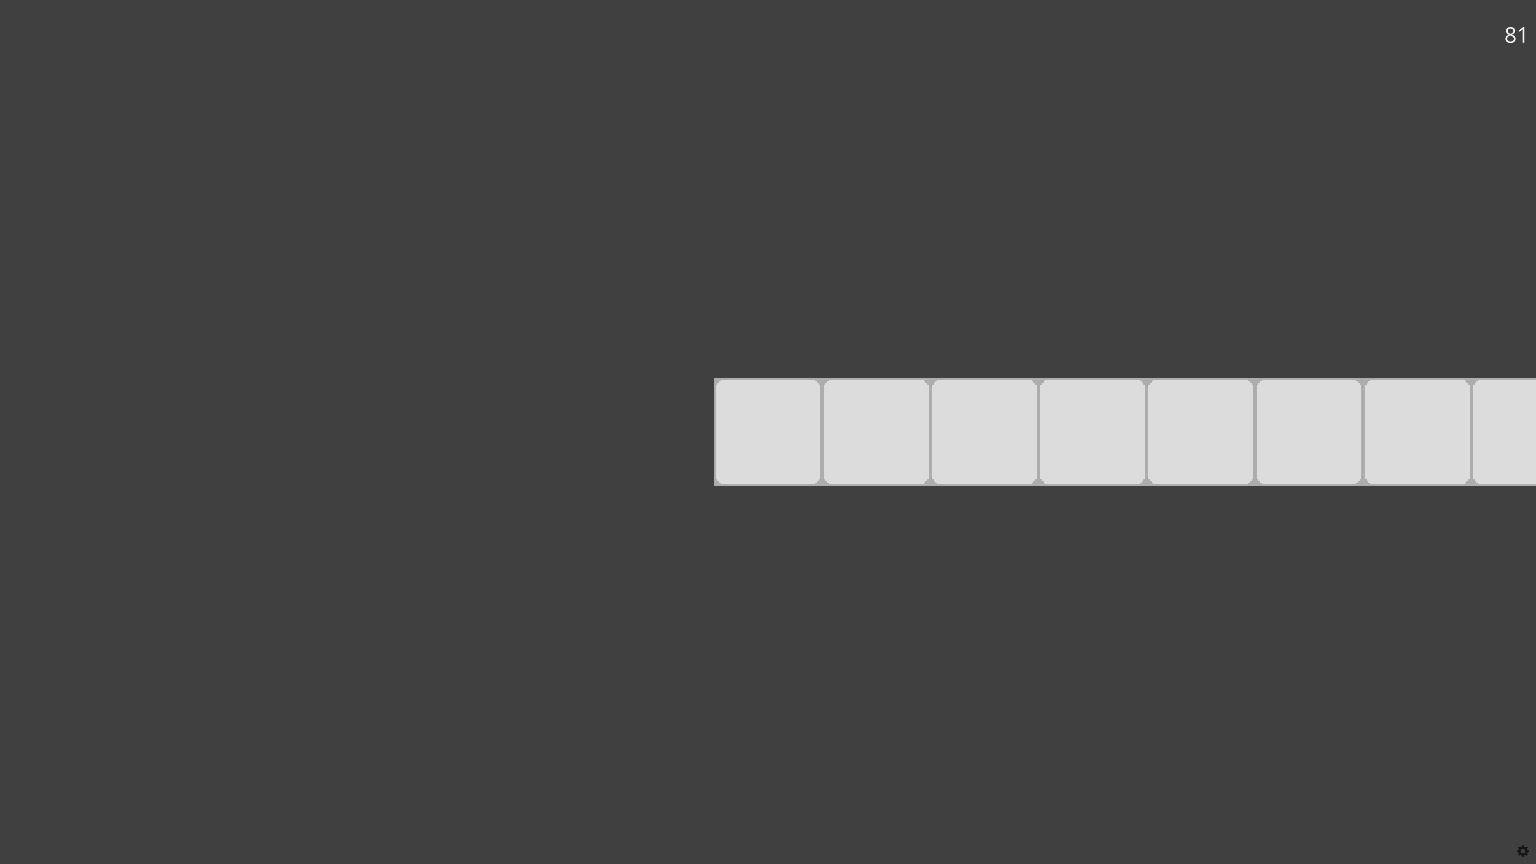
\includegraphics[width=\textwidth]{img/2.png}
    \end{frame}


    \subsection{FirstPersonController}
    \begin{frame}{Определение}
        \begin{justify}
            Программа покажет на экране плоское изображение. Для просмотра блочной сцены в 3D нужен наблюдатель. Его можно создать с помощью готового объекта \textbf{FirstPersonController}.
        \end{justify}
    \end{frame}

    \begin{frame}[fragile]{Код}
        \frametitle{Код}
        \scriptsize
        \rule{\textwidth}{1pt}
        \begin{minted}[autogobble]{python}
            # Прошлый код
            ...
            
            # Создаем объект player, который представляет собой контроллер 
            # от первого лица (FirstPersonController) - специальный класс 
            # для управления персонажем в 3D-играх
            player = FirstPersonController()
            
            # Устанавливаем свойство gravity объекта player равным 0.0, 
            # что означает, что персонаж не подвержен гравитации и не падает вниз
            player.gravity = 0.0
            
            # Запускаем проект
            app.run()
        \end{minted}
        \rule{\textwidth}{1pt}
    \end{frame}
    
    \begin{frame}{Результат}
        \begin{center}
            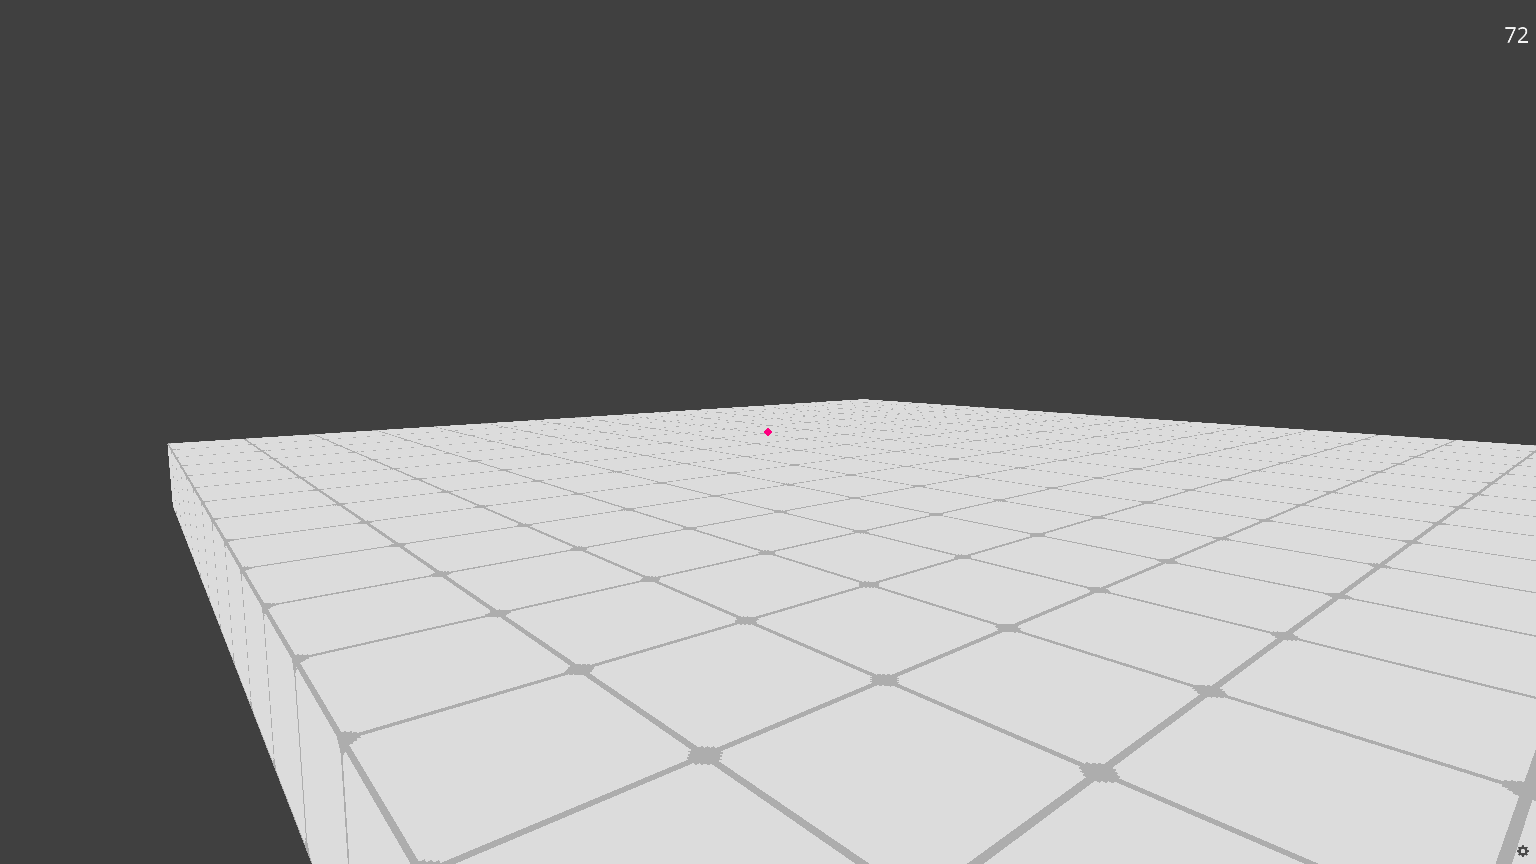
\includegraphics[width=0.7\textwidth]{img/3.png}
        \end{center}
        \begin{justify}
            \textit{Игроком по умолчанию можно управлять с помощью мышки и кнопок W, A, S, D. Но есть особенность: если переключиться на русскую раскладку, то при нажатии кнопки возникнет ошибка. Не забудь переключить раскладку!}
        \end{justify}
    \end{frame}


    \subsection{Текстурирование блоков}
    \begin{frame}{Определение}
        \begin{justify}
            Для начала стоит создать и раскрасить блоки. Нужно сначала сделать модель в Blender, потом подготовить текстуру и затем импортировать объект в программу. 
            Мы же возьмем уже готовые объект и текстуру.
            
            Модель блока находится в папке \texttt{models} под названием \texttt{block.obj}, а текстура травы для него - в папке \texttt{textures} под названием \texttt{grass.png}. Если хочешь, можешь взять и другую текстуру из находящихся в этой папке, кроме \texttt{arm.png}.
            
            Для начала создадим переменную с нашей загруженной текстурой, а затем будет использовать её и нашу модель \texttt{block} при создании объектов \texttt{Entity} в циклах.
        \end{justify}
    \end{frame}

    \begin{frame}[fragile]{Код}
        \frametitle{Код}
        \scriptsize
        \rule{\textwidth}{1pt}
        \begin{minted}[autogobble]{python}
            # Прошлый код
            ...
            
            # загружаем текстуру
            grass_texture = load_texture('assets/grass.png')
            
            # Создаем двойной цикл for, который повторяется 16 раз по переменным x и z
            for x in range(16): 
            	for z in range(16):
            	    # Создаем сущность в виде БЛОКА с НАШЕЙ текстурой 
                        # и задаем ей позицию в пространстве по координатам x, 0 и z
            	    Entity(model='models/block', scale=0.5, texture=grass_texture, 
                        position=(x, 0, z))
            
            ...
            # Прошлый код
            
            # Запускаем проект
            app.run()
        \end{minted}
        \rule{\textwidth}{1pt}
    \end{frame}
    
    \begin{frame}{Результат}
        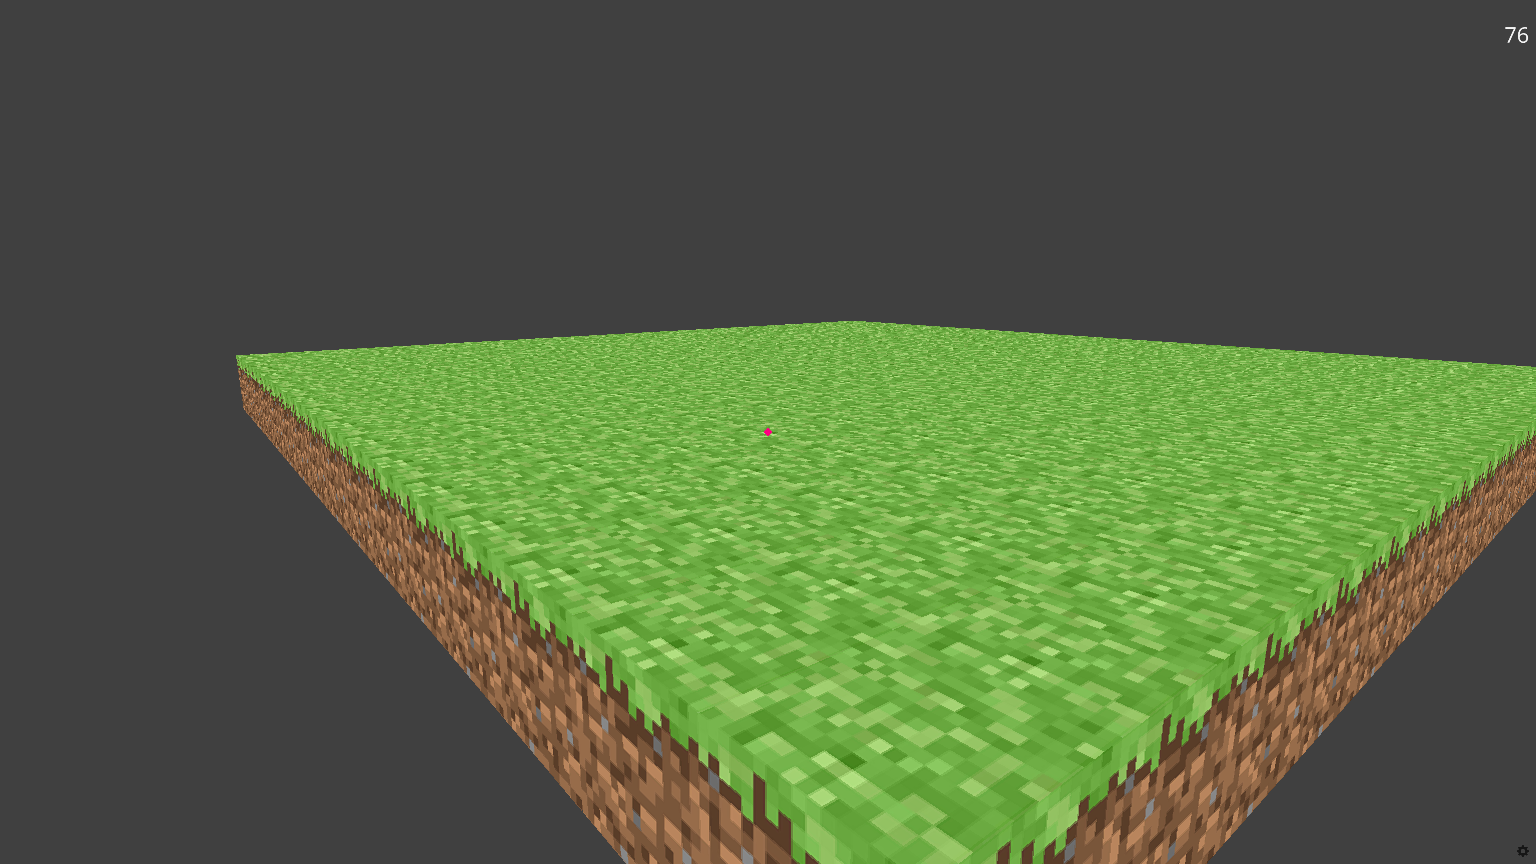
\includegraphics[width=\textwidth]{img/4.png}
    \end{frame}


    \subsection{Текстурирование персонажа}
    \begin{frame}{Определение}
        \begin{justify}
            Так же можно сделать и руку персонажа. Сперва — подготовить текстуру для модели в Blender, потом — привести ее в программу через \texttt{Entity}. Чтобы прикрепить руку к камере персонажа, нужно настроить параметры — положение и угол.
            Мы же снова воспользуемся готовыми объектом и текстурой руки.
        
            Как и раньше, модель руки находится \texttt{models/arm.obj}, а текстура - \texttt{textures/arm.png}.
        \end{justify}
    \end{frame}

    \begin{frame}[fragile]{Код}
        \scriptsize
        \rule{\textwidth}{1pt}
        \begin{minted}[autogobble]{python}
            # Прошлый код
            ...
            # ЗДЕСЬ ФУНКЦИЯ input
            
            # Загружаем текстуру для руки
            arm_texture = load_texture("textures/arm.png")
            # Создаем сущность в виде руки и присваиваем ее переменной hand
            hand = Entity(
            	# Указываем камеру, чтобы рука всегда была видна на экране
            	parent=camera.ui,
            	# Указываем модель
            	model="models/arm",
            	# Указываем текстуру
            	texture=arm_texture,
            	# Указываем масштаб сущности как 0.2, чтобы рука не была слишком большой или маленькой
            	scale=0.2,
            	# Указываем поворот
            	rotation=Vec3(150, -10, 0),
            	# Указываем позицию
            	position=Vec2(0.6, -0.6),
            )
            
            ...
            # Прошлый код
        \end{minted}
        \rule{\textwidth}{1pt}
    \end{frame}
    
    \begin{frame}{Результат}
        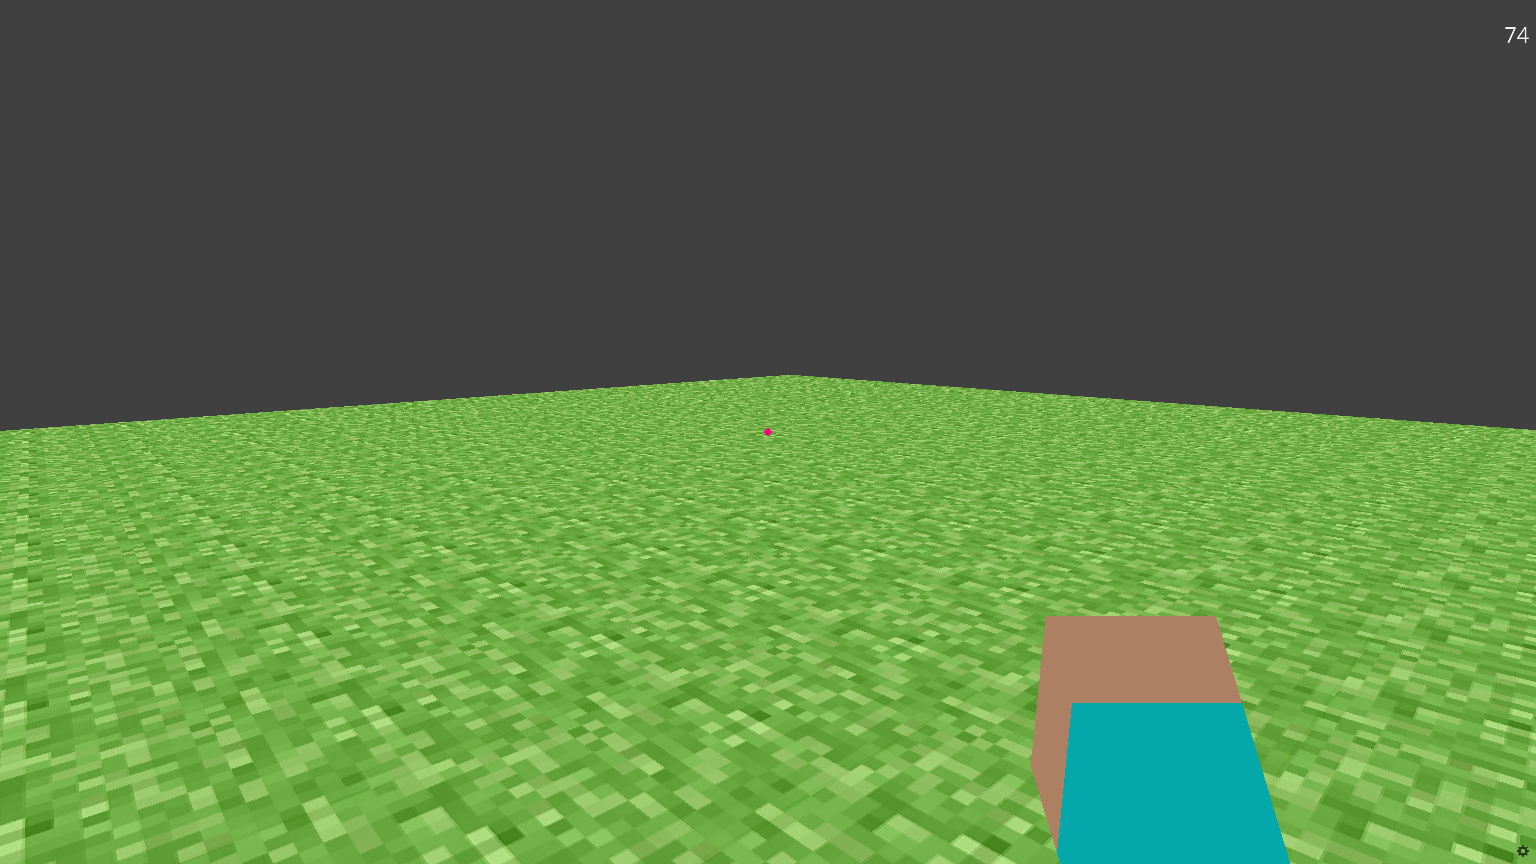
\includegraphics[width=\textwidth]{img/5.png}
    \end{frame}


    \subsection{Текстурирование неба}
    \begin{frame}{Определение}
        \begin{justify}
            \texttt{Entity} поможет сделать небо — достаточно создать модель сферы с текстурой неба и ее использовать.
            
            Как и раньше, текстура неба - \texttt{textures/sky.png}.
        \end{justify}
    \end{frame}

    \begin{frame}[fragile]{Код}
        \scriptsize
        \rule{\textwidth}{1pt}
        \begin{minted}[autogobble]{python}
            # Прошлый код
            ...
            # ЗДЕСЬ КОД ДЛЯ РУКИ HAND
            
            # Загружаем текстуру
            sky_texture = load_texture("textures/sky.png")
            
            # Создаем сущность в виде неба и присваиваем ее переменной sky
            sky = Entity(
            	# Указываем модель сферы
            	model="sphere",
            	# Указываем текстуру
            	texture=sky_texture,
            	# Указываем масштаб, чтобы небо было достаточно большим
            	scale=1000,
            	# Указываем, чтобы текстура неба была видна с обеих сторон сферы
            	double_sided=True,
            )
            ...
            # Прошлый код
        \end{minted}
        \rule{\textwidth}{1pt}
    \end{frame}
    
    \begin{frame}{Результат}
        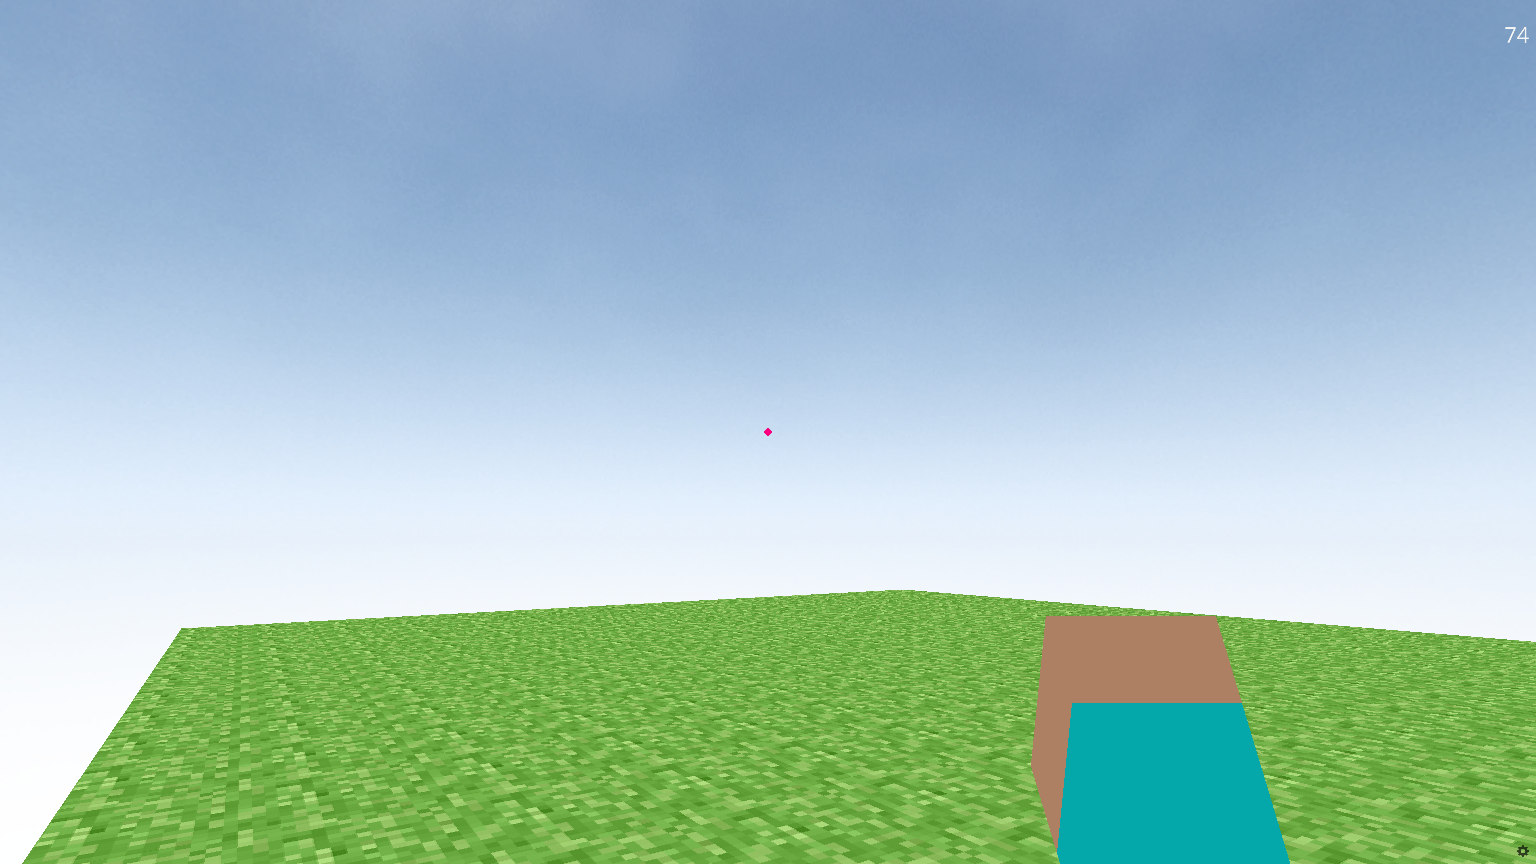
\includegraphics[width=\textwidth]{img/6.png}
        \begin{center}
            \textit{Получаем красивое небо!}
        \end{center}
    \end{frame}


    \subsection{Включение блоков Button}
    \begin{frame}{Определение}
        \begin{justify}
            Некоторые блоки нельзя «ломать». Чтобы сделать игру интерактивной, нужен особый объект Button. Он умеет работать с функцией input и методом destroy, которые помогают разбивать блоки. Создадим свой собственный класс таких блоков на основе Button. Добавим так же звуковое сопровождение для установки и удаления блока.
        \end{justify}
    \end{frame}

    \begin{frame}[fragile]{Код}
        \scriptsize
        \rule{\textwidth}{1pt}
        \begin{minted}[autogobble]{python}
            # Прошлый код
            ...
            # Загружаем звук
            punch_sound = Audio("sounds/punch.wav", loop=False, autoplay=False)
            
            # Создаем класс Voxel, специальный класс для создания интерактивных объектов
            class Voxel(Button):
            	# Определяем конструктор
            	def __init__(self, position=(0, 0, 0), texture=grass_texture):
            		super().__init__(
            			# Указываем сцену, чтобы объект был виден в игре
            			parent=scene,
            			# Указываем модель объекта
            			model="models/block",
            			# Указываем масштаб объекта
            			scale=0.5,
            			# Указываем текстуру объекта
            			texture=texture,
            			# Указываем позицию объекта
            			position=position,
        \end{minted}
        \rule{\textwidth}{1pt}
    \end{frame}

    \begin{frame}[fragile]{Код}
        \scriptsize
        \rule{\textwidth}{1pt}
        \begin{minted}[autogobble]{python}
            			origin_y=0.5, # Указываем точку опоры объекта
            			# Указываем цвет объекта как случайный оттенок зеленого
            			color=color.color(0, 0, random.uniform(0.9, 1)),
            		)
            	# Определяем метод input класса, который принимает один параметр: key
            	def input(self, key):
            		# Проверяем, наведен ли курсор мыши на объект
            		if self.hovered:
            			# Проверяем, нажата ли правая кнопка мыши
            			if key == "right mouse down":
            				punch_sound.play() # Воспроизводим звук
            				# Создаем объект Voxel с текстурой и позицией
            				Voxel(position=self.position + mouse.normal, 
                                texture=grass_texture)
            			# Проверяем, нажата ли левая кнопка мыши
            			if key == "left mouse down":
            				punch_sound.play() # Воспроизводим звук
            				# Уничтожаем текущий объект
            				destroy(self)ё
        \end{minted}
        \rule{\textwidth}{1pt}
    \end{frame}

    \begin{frame}[fragile]{Код}
        \scriptsize
        \rule{\textwidth}{1pt}
        \begin{minted}[autogobble]{python}
            # Создаем двойной цикл for, который повторяется 16 раз по переменным x и z
            for x in range(16):
            	for z in range(16):
            		# Создаем объект Voxel с текстурой grass_texture
                        # и позицией по координатам x и z
            		Voxel(position=(x, 0, z))
        \end{minted}
        \rule{\textwidth}{1pt}
    \end{frame}
    
    \begin{frame}{Результат}
        \begin{center}
            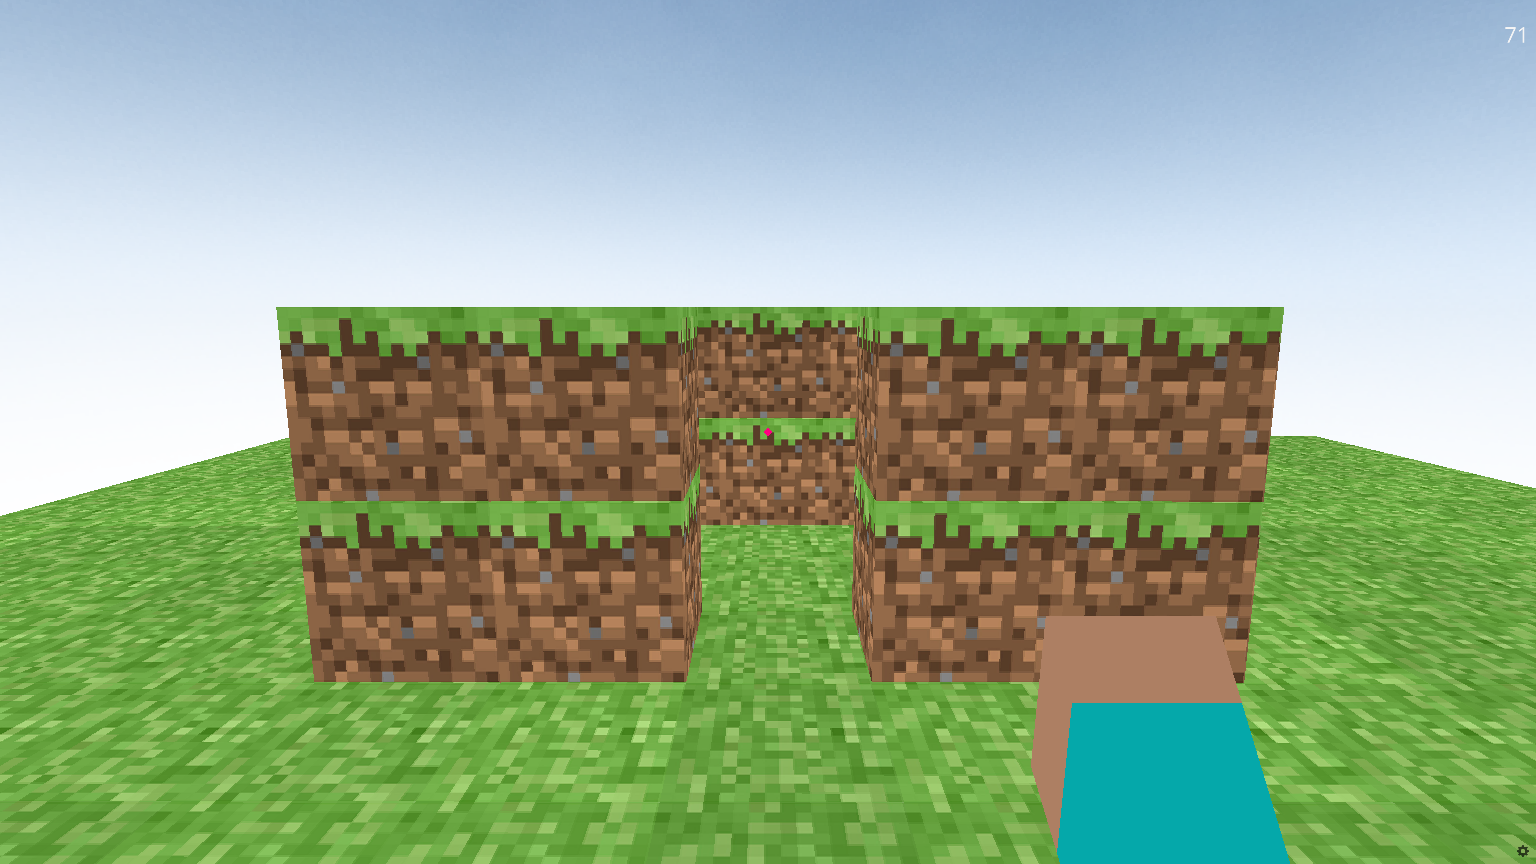
\includegraphics[width=0.9\textwidth]{img/7.png} \\
            \begin{justify}
                \textit{Теперь можно строить! Чтобы персонаж мог прыгать, убери строку \texttt{player.gravity = 0.0}!}
            \end{justify}
        \end{center}
    \end{frame}


    \subsection{Генерация мира}
    \begin{frame}{Шум Перлина в Minecraft}
        \begin{columns}
            \begin{column}{0.7\textwidth}
                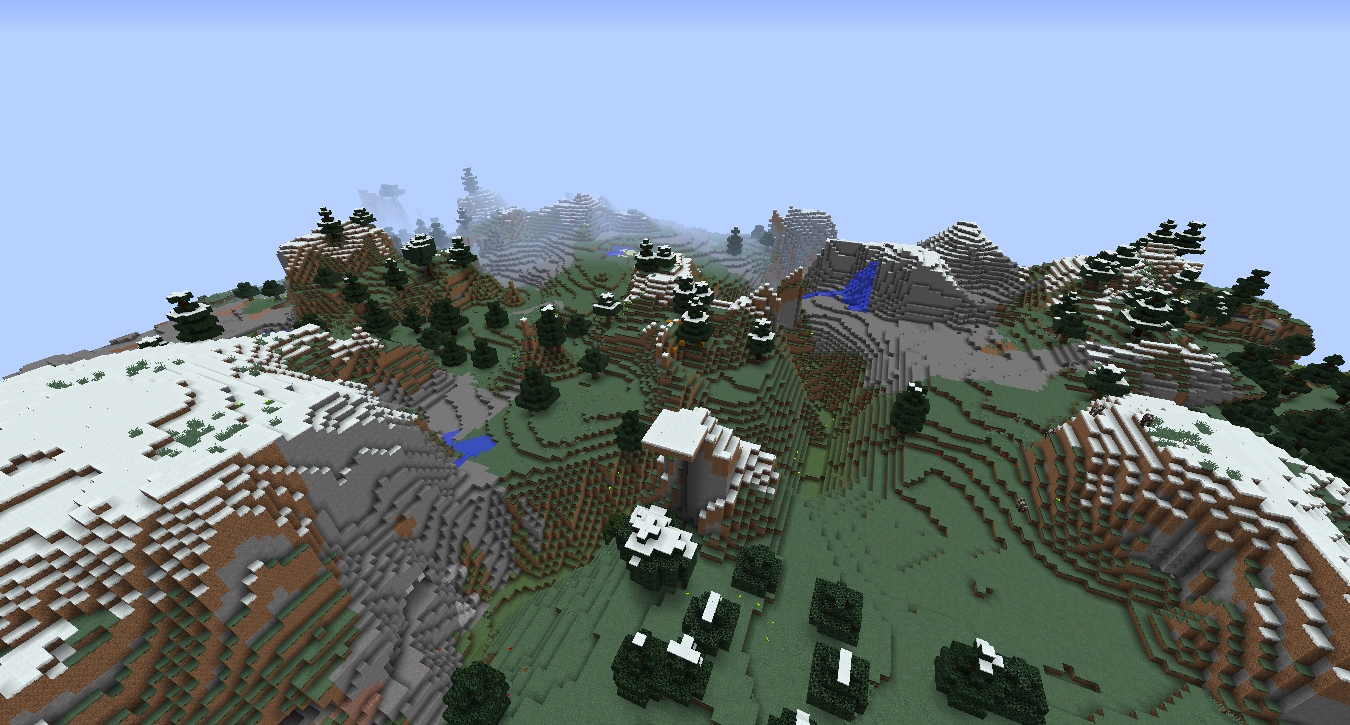
\includegraphics[width=\textwidth]{img/mine_perlin_noise.png}
            \end{column}
            \begin{column}{0.3\textwidth}
                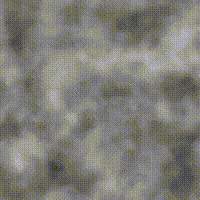
\includegraphics[width=\textwidth]{img/AggravatingThoseArieltoucan-0.png}
            \end{column}
        \end{columns}
        \begin{justify}
            В основе генерации мира Minecraft лежат шумы Перлина — алго ритм для генерации объёмных ландшафтов. Генератором создаётся карта шумов — или, грубо говоря, карта высот. Её можно сравнить с топографической картой: там, где светлее — местность выше, там, где темнее — ниже.
        \end{justify}
    \end{frame}
    

    \begin{frame}{Шум Перлина}
        \begin{justify}
            Шум Перлина — это способ процедурной генерации по псевдослучайному алгоритму. Принцип такой: вы вводите число seed, на основе которого создается текстура поверхности.
            При одинаковом значении seed шум не изменится, если не настроить внутренние параметры алгоритма.
        \end{justify}
        \begin{center}
            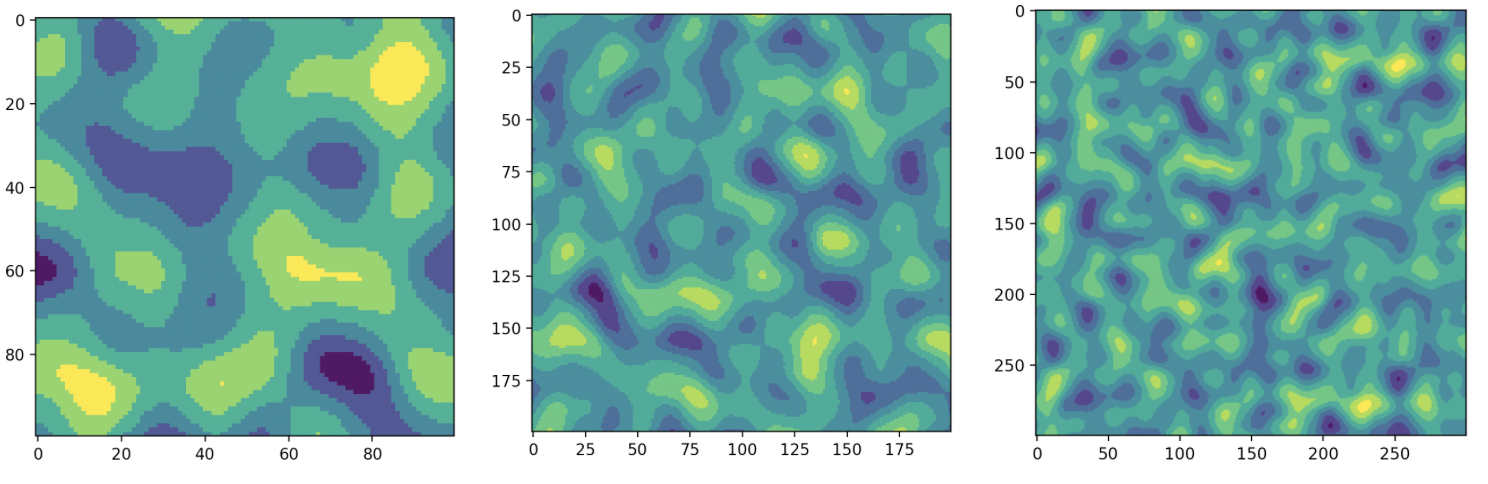
\includegraphics[width=0.7\textwidth]{img/perlin_noise.png}
        \end{center}
    \end{frame}

    \begin{frame}
        \frametitle{Шум Перлина}
        \begin{justify}
            Попробуем сгенерировать шумы Перлина!\\
            Откроем \texttt{perlin\_test.py} и попробуем запускать код, при этом меняя значение \texttt{seed=*твое число*}!
            Так же можно изменять значение \texttt{terrain\_width} (размер шума) и \texttt{octaves} (насколько часто меняется высота).
        \end{justify} \\
        \begin{center}
            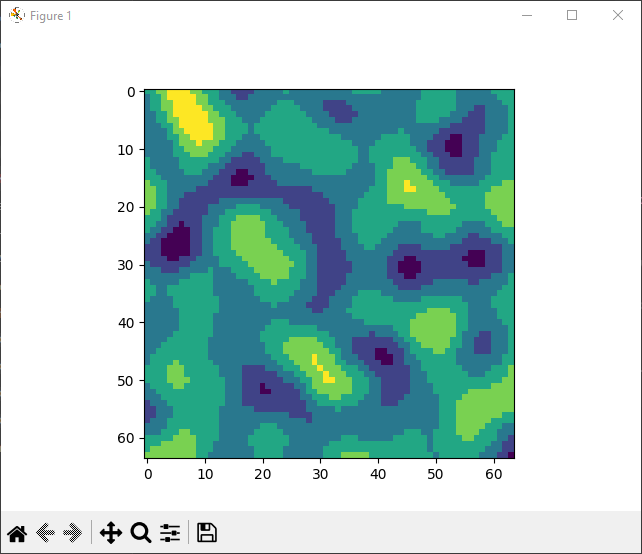
\includegraphics[width=0.3\textwidth]{img/perlin_test.png} \\ 
            Пример работы программы: \texttt{octaves = 2, seed = 2023, terrain\_width = 64}
        \end{center}
    \end{frame}

    \begin{frame}[fragile]{Код}
        \scriptsize
        \rule{\textwidth}{1pt}
        \begin{minted}[autogobble]{python}
            from numpy import floor # НЕОБХОДИМО ДОБАВИТЬ!
            from perlin_noise import PerlinNoise # НЕОБХОДИМО ДОБАВИТЬ!
            ...
            # Прошлый код
            ...
            # Создаем объект noise - шум Перлина
            noise = PerlinNoise(octaves=2, seed=2023)
            # Создаем переменную am которая определяет амплитуду шума
            amp = 6
            # Создаем переменную, которая определяет частоту шума
            freq = 24
            # Указываем ширину и длину 
            terrain_width = 30
        \end{minted}
        \rule{\textwidth}{1pt}
    \end{frame}

    \begin{frame}[fragile]{Код}
        \scriptsize
        \rule{\textwidth}{1pt}
        \begin{minted}[autogobble]{python}
            # Создаем двумерный список landscale, который будет хранить высоты блоков
            landscale = [[0 for i in range(terrain_width)] for i in range(terrain_width)]
            
            # Создаем цикл for, который перебирает все позиции блоков
            for position in range(terrain_width**2):
                # Вычисляем координату x 
                x = floor(position / terrain_width)
                # Вычисляем координату z 
                z = floor(position % terrain_width)
                # Вычисляем координату y
                # Для получения значения шума Перлина используем метод noise
                y = floor(noise([x / freq, z / freq]) * amp)
            
                # Присваиваем значение y в списке landscale по индексам x и z
                landscale[int(x)][int(z)] = int(y)
        \end{minted}
        \rule{\textwidth}{1pt}
    \end{frame}


    \begin{frame}[fragile]{Код}
        \scriptsize
        \rule{\textwidth}{1pt}
        \begin{minted}[autogobble]{python}
            # Создаем двойной цикл for, который перебирает все координаты x и z
            for x in range(terrain_width):
                for z in range(terrain_width):
                    # Создаем объект block класса Voxel, 
                    # который представляет собой интерактивный блок в игре
                    # Указываем параметры блока, такие как позицию по трем осям (x, y и z), используя значение y из списка landscale по индексам x и z
                    block = Voxel(position=(x, landscale[x][z], z))
            ...
            # Прошлый код
        \end{minted}
        \rule{\textwidth}{1pt}
    \end{frame}

    \begin{frame}{Результат}
        \begin{center}
            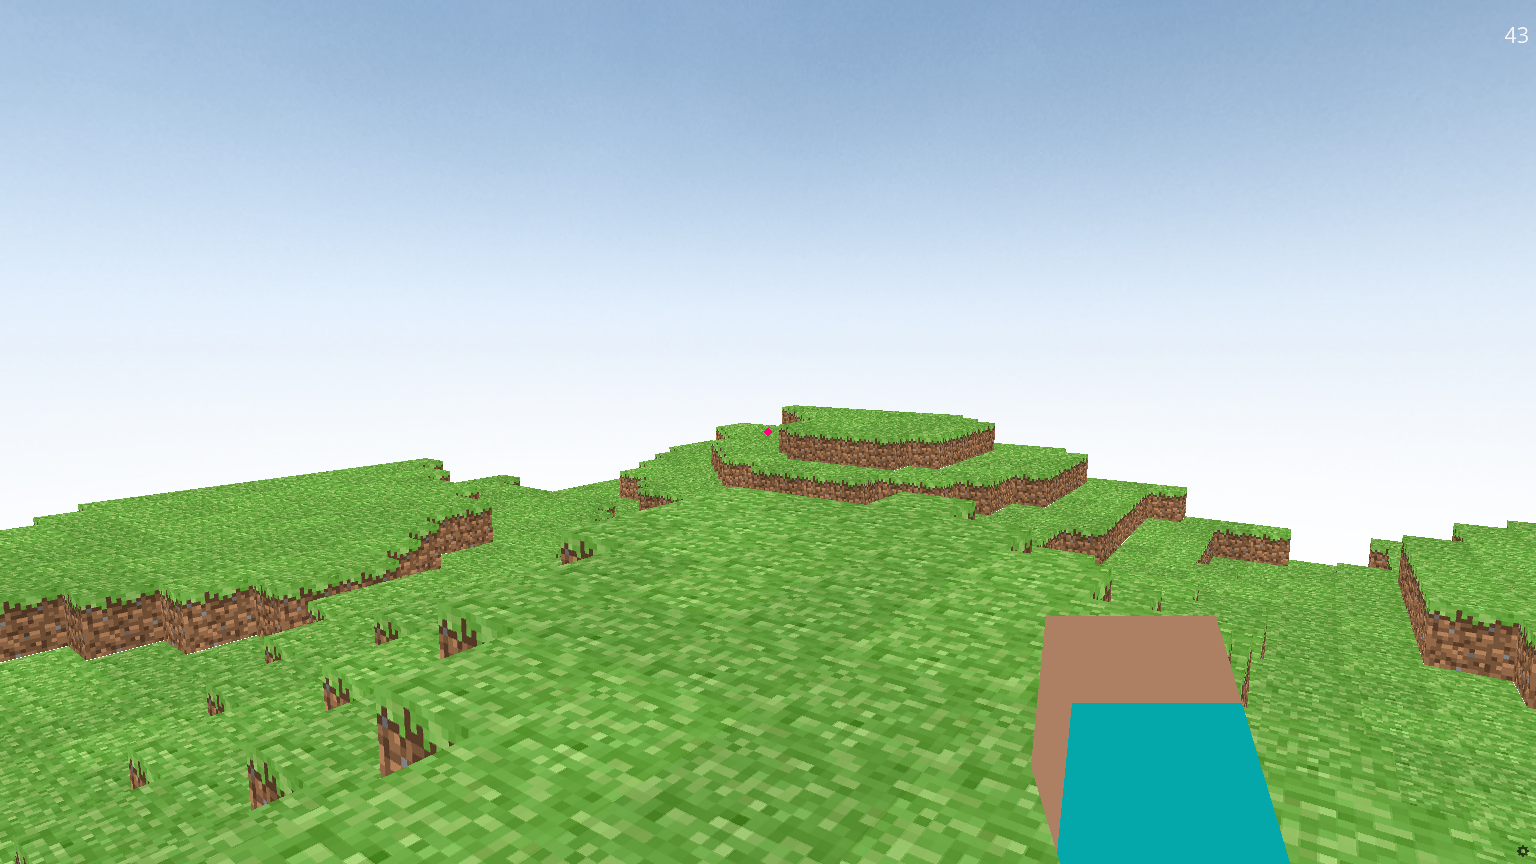
\includegraphics[width=0.85\textwidth]{img/8.png} \\
            \begin{justify}
                \textit{Теперь мир не просто плоский! \\ Таким же способом можно создавать и рудники. Только для них применяются черви Перлина.}
            \end{justify}
        \end{center}
    \end{frame}


    \subsection{Последние штрихи}
    \begin{frame}{Добавление различных блоков}
        \begin{justify}        
            Строить одним видом блоком, конечно же, неинтересно, поэтому давай добавим ещё 4 разных вида блоков: земля, камень, кирпичи и доски.
    
            Для этого создадим переменную \texttt{block\_pick} в которой будет содержаться номер того предмета, который мы будем устанавливать. Изменять значение будем с помощью цифр от 1 до 5.
    
            Кроме того, необходимо загрузить текстуры для других блоков.
        \end{justify}  
    \end{frame}


    \begin{frame}[fragile]{Код}
        \scriptsize
        \rule{\textwidth}{1pt}
        \begin{minted}[autogobble]{python}
            # Прошлый код
            ...
            block_pick = 1 # Создаем переменную хранит номер выбранного блока
            # Определяем функцию input с одним параметром key
            def input(key):
            	# Объявляем, что мы будем использовать переменную block_pick
            	global block_pick
            	# Проверяем, равна ли переменная key строке "q" или "escape"
            	if key == "q" or key == "escape":
            		quit() # Если да, то завершаем программу
            	if key == "1": # Трава
            		block_pick = 1
            	if key == "2": # Земля
            		block_pick = 2
            	if key == "3": # Камень
            		block_pick = 3
            	if key == "4": # Кирпичи
            		block_pick = 4
            	if key == "5": # Доски
            		block_pick = 5
            ...
            # Прошлый код
        \end{minted}
        \rule{\textwidth}{1pt}
    \end{frame}
    

    \begin{frame}[fragile]{Код}
        \scriptsize
        \rule{\textwidth}{1pt}
        \begin{minted}[autogobble]{python}
            # Создаем класс Voxel, специальный класс для создания интерактивных объектов
            class Voxel(Button):
            	# Определяем конструктор
            	def __init__(self, position=(0, 0, 0), texture=grass_texture):
            		super().__init__(
            			# Указываем сцену, чтобы объект был виден в игре
            			parent=scene,
            			# Указываем модель объекта
            			model="models/block",
            			# Указываем масштаб объекта
            			scale=0.5,
            			# Указываем текстуру объекта
            			texture=texture,
            			# Указываем позицию объекта
            			position=position,
            			# Указываем точку опоры объекта
            			origin_y=0.5,
            			# Указываем цвет объекта как случайный оттенок зеленого
            			color=color.color(0, 0, random.uniform(0.9, 1)),
            		)
        \end{minted}
        \rule{\textwidth}{1pt}
    \end{frame}


    \begin{frame}[fragile]{Код}
        \scriptsize
        \rule{\textwidth}{1pt}
        \begin{minted}[autogobble]{python}
        # Определяем метод input класса, который принимает один параметр: key
        def input(self, key):
            # Проверяем, наведен ли курсор мыши на объект
            if self.hovered:
                # Проверяем, нажата ли правая кнопка мыши
                if key == "right mouse down":
                    # Воспроизводим звук
                    punch_sound.play()
                    # Создаем объект Voxel с нужной текстурой и позицией
                    if block_pick == 1:
                        Voxel(position=self.position+mouse.normal, texture=grass_texture)
                    if block_pick == 2:
                        Voxel(position=self.position+mouse.normal, texture=dirt_texture)
                    if block_pick == 3:
                        Voxel(position=self.position+mouse.normal, texture=stone_texture)
                    if block_pick == 4:
                        Voxel(position=self.position+mouse.normal, texture=brick_texture)
                    if block_pick == 5:
                        Voxel(position=self.position + mouse.normal, texture=wood_texture)
        \end{minted}
        \rule{\textwidth}{1pt}
    \end{frame}

    \begin{frame}[fragile]{Код}
        \scriptsize
        \rule{\textwidth}{1pt}
        \begin{minted}[autogobble]{python}
            # Проверяем, нажата ли левая кнопка мыши
                    if key == "left mouse down":
                        # Воспроизводим звук
                        punch_sound.play()
                        # Уничтожаем текущий объект
                        destroy(self)
        \end{minted}
        \rule{\textwidth}{1pt}
    \end{frame}

    \begin{frame}{Результат}
        \begin{center}
            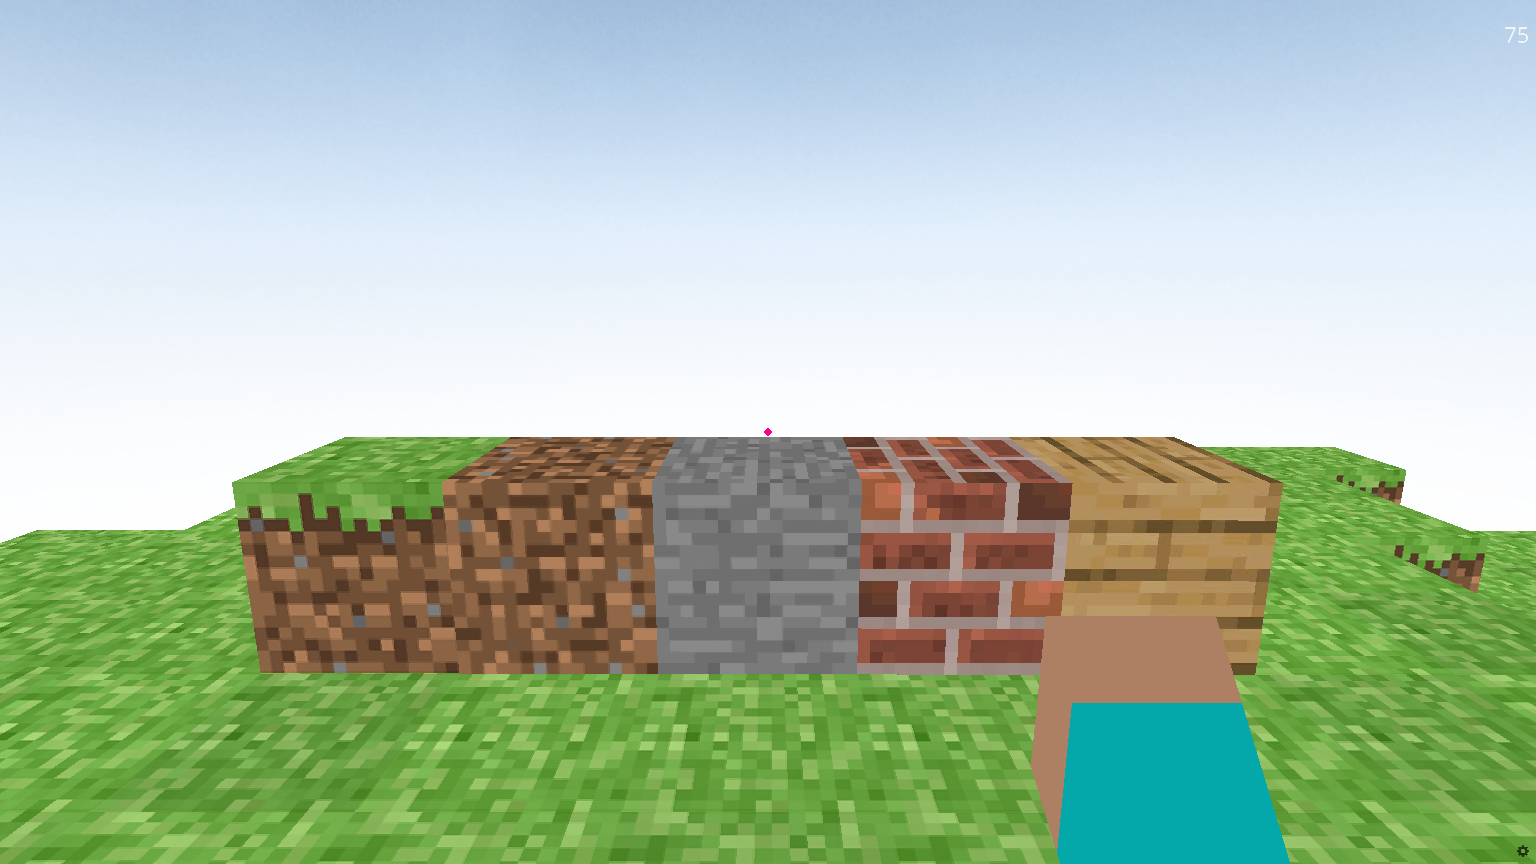
\includegraphics[width=0.85\textwidth]{img/9.png} \\
            \begin{justify}
                \textit{Наш клон Minecraft готов!}
            \end{justify}
        \end{center}
    \end{frame}

    % \begin{frame}[fragile]{Код}
    %     \scriptsize
    %     \rule{\textwidth}{1pt}
    %     \begin{minted}[autogobble]{python}
            
    %     \end{minted}
    %     \rule{\textwidth}{1pt}
    % \end{frame}
    
    \section{Примечания}
    \begin{frame}{Примечания}
        \footnotesize{
            \begin{thebibliography}{99}
            
            \bibitem[ursina]{p1} Ursina Engine
            \newblock \href{https://www.ursinaengine.org/}{https://www.ursinaengine.org/}
            
            \bibitem[github]{p2} Репозиторий проекта
            \newblock \href{https://github.com/L4zzur/minecraft-on-ursina}{https://github.com/L4zzur/minecraft-on-ursina}
            
            \end{thebibliography}
        }
    \end{frame}

    \section{Титульный лист}
	\begin{frame}
		\titlepage
	\end{frame}

\end{document}